%!TEX root = rapport.tex
This section will present implementation details on how the heap has
been implemented, and why these choices were made. Also the details of
all the implemented streams are discussed.

We define the following:
\begin{itemize}
  \item $V$ is the maximal number of elements in a node. Hence, a
    node is imperfect if it contains $< \left\lceil \frac{V}{2}
    \right\rceil$ elements.
  \item $d$ is the fan-out of the tree.
\end{itemize}

\subsection{Heap}
In the paper the structure of the heap was represented using pointers,
such that every node stores pointers to its children and its
parent. Instead, we have chosen to embed the structure of the heap
inside an array, such that an array entry contains a reference to a
node in the heap. Then the index of the parent node and the indices of
the child node can be calculated using simple integer operations, and
the corresponding node can be found by looking up in the node array.

Using this representation, it is also very easy to swap the position
of two nodes, as the two entries in the array can simply be swapped
(this is required in the insert operation when the last node is
imperfect).

To store the elements of the heap, a big file have been allocated on
disk. This file is (virtually) divided into blocks of size $V$, such
that each block is associated with a node in the tree.

When elements are inserted into the heap, they file may become too
small. Hence when a new block is added, and the file does not have
enough space, the file is extended by $V$ elements. Growing the file
should be handled by the operating system using only constant IOs, and
hence there should be no problem in growing the file every time a new
node is added. As we have enough disk space, we have chosen not to
shrink the file when extracting elements. Again since it should only
require a constant number of IOs we do not believe this will have any
significant influence on our benchmarks.

Every node in the tree has an associated stream, which can read and
write the block associated to the node. Unless mentioned otherwise
in the stream section, the stream for a given node is opened and
closed as it is needed. That is, every time an element should be read
and written, the stream is opened, the operations are executed on the
stream, and then the stream is closed again. This also means that at
most $d + 1$ streams are active at the same time, which happens in
the refill operation.

\begin{figure}
  \centering
  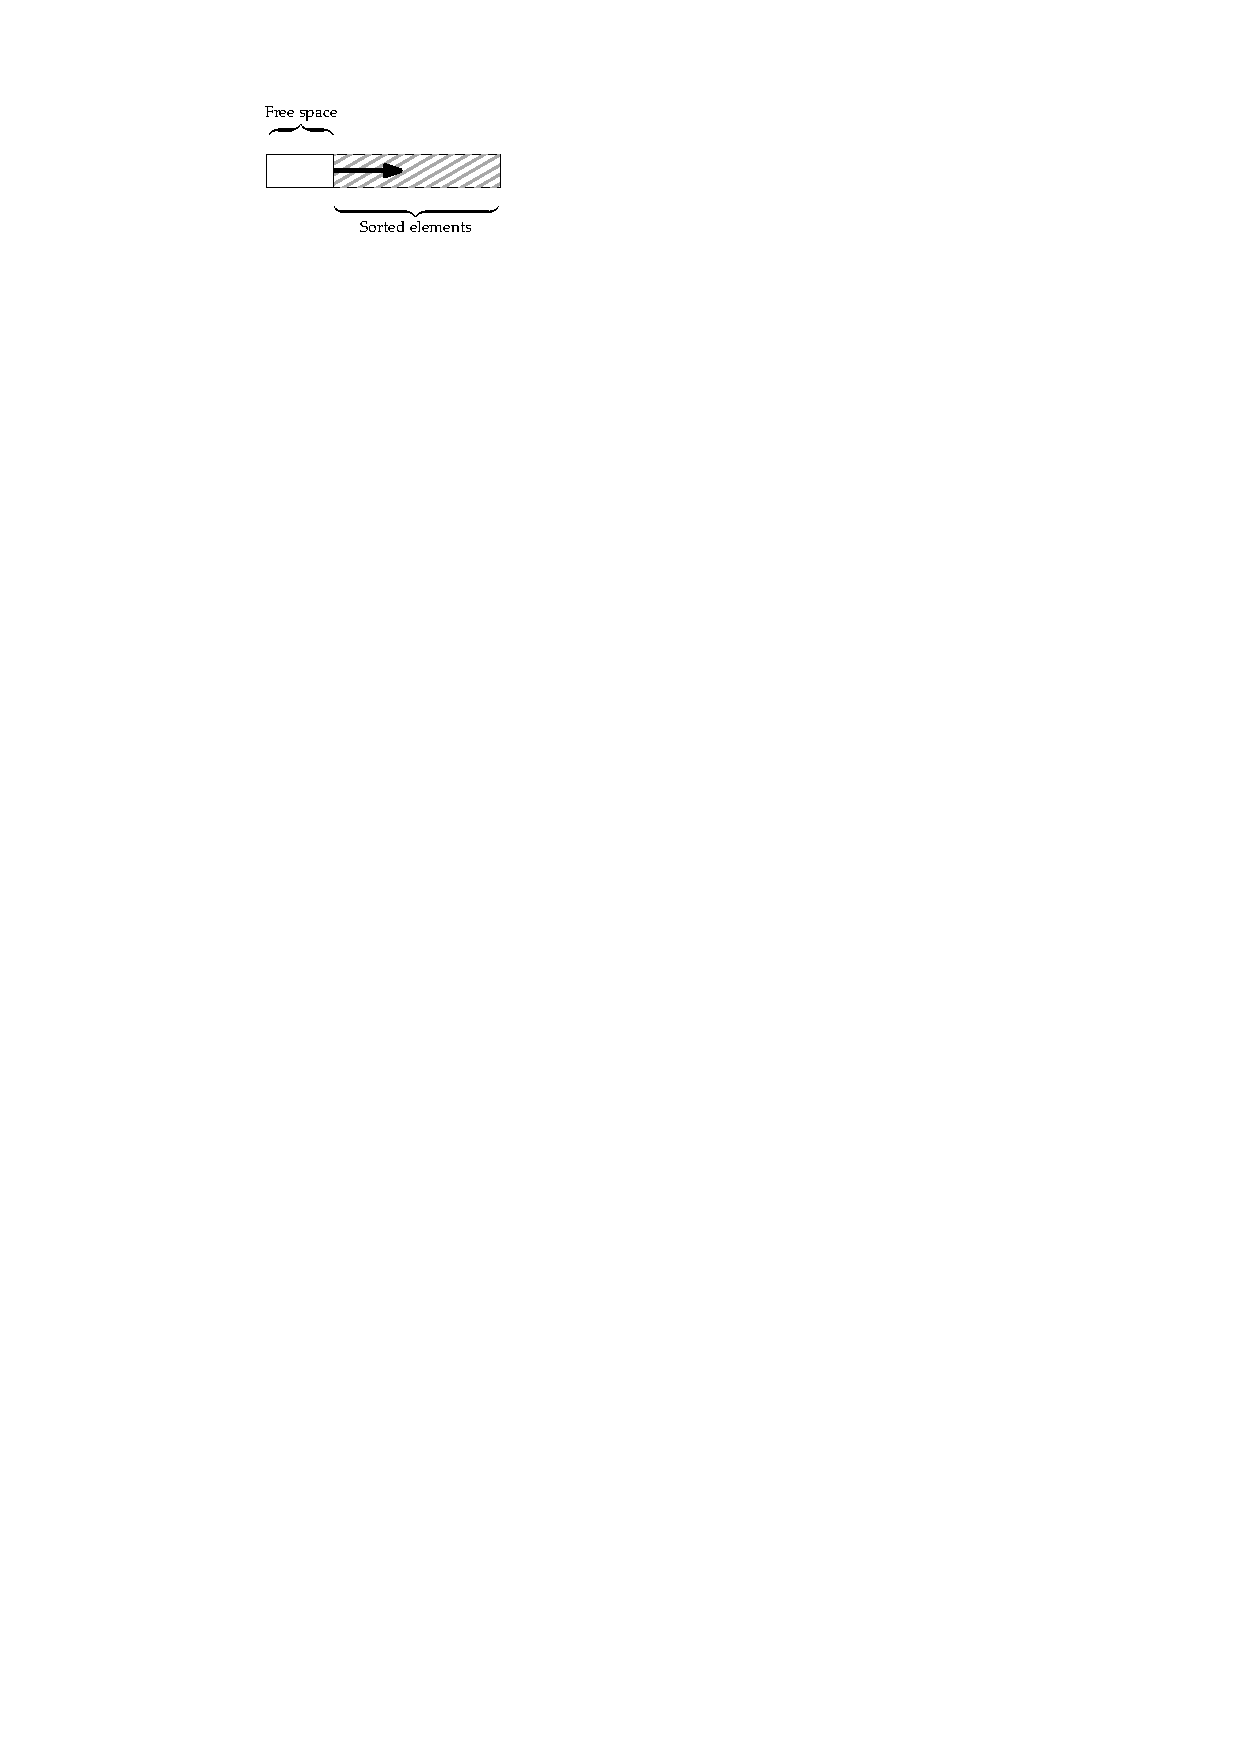
\includegraphics[width=6cm]{node_block}
  \caption{Layout of a block associated with a node. Elements are
    stored in decreasing sorted order, and is placed as far to the
    right as possible.}
  \label{fig:node-block}
\end{figure}

Inside a block, elements are stored to the right in the block in
descending sorted order, as illustrated by
Figure~\ref{fig:node-block}. This layout facilitates forward reading
when extracting the maximum element.

\subsubsection{Sifting}
\label{sec:heap:sifting}
When doing the sift operation, it is required to merge blocks of the
current node and its parent. When doing this, one should be careful
about how many elements are assigned to respectively the parent and
the current node after the merge: If too many elements are transferred
to the parent, such that an element with strictly lower priority is
added to the parent, then the heap invariant between the parent and
its other children may be violated.

On the other hand, it is desired to assign as many elements as
possible to the parent node, as this may delay future refill
operations.

In the paper they assign $\max(r - h, \ceil*{\frac{V}{2}})$ elements to
the child, where $r$ is the sum of the number of elements in the
parent and in the current node, and $h$ is the number of elements
having priority higher than or equal to the parent node. On counter
example to this strategy is when two full blocks are merged, and $h =
0$ (that is, all the child nodes are smaller than the parent node),
then all elements will be assigned to the child, which renders the
parent node imperfect.

We have fixed this by per default to assign
\[
  \max \left( \text{child elements less than minimum in parent}, \ceil*{\frac{V}{2}} \right)
\]
elements to the child. But then it might be the parent gets
overfilled, in which case a sufficient number of the smallest elements
from the parent are transferred to the child node. By construction
this division will satisfy the invariants of the heap.
\\
\\
Two implementations have been made for merging a block:
\begin{description}
\item[Memory inefficient] version where $2V$ elements are buffered,
  and the merging is done in internal memory. This approach has the
  advantage that it only reads forward.
\item[Memory efficient] version where only $V$ elements are
  buffered. The problem with this implementation is to determine how
  many elements should go to the child and to the parent, without
  reading the unbuffered block several times.

  In order to get around this problem, the minimum element in all
  nodes have been cached, which means that the number of elements
  going to the current node (and the parent) can be computed when
  reading the elements of the current node into the buffer. Then the
  elements going to the current node can be written backwards into its
  block, by also reading the buffer and the block of the parent node
  backwards.
\end{description}
We have chosen to investigate both techniques, as we are unsure what
the penalty of reading and writing backwards is, due to read-ahead
etc.. We believe the effect will be different for different types of
streams, as some with large buffers or memory mapped files, may handle
the situation in a better way.

\subsubsection{Verifying correctness}
To ensure the correctness of our heap implementation, the following
three techniques have been used:
\begin{itemize}
\item A graphical representation of the data structure have been
  implemented, enabling us to manually verify small test inputs.
\item A consistency check function has been implemented, which is
  called after every insert and extract operation. The consistency
  check function makes a recursive decent of the nodes in the heap,
  and check that all invariants are satisfied.
\item A sanity test function have been made, where $1\cdot 10^6$
  uniformly random integers was inserted into the heap, and then
  extracted afterwards. It was tested that the integers came out in
  sorted order.
\end{itemize}
All of the above checks passes in our implementation, and we have no
knowledge of bugs.

\subsection{Streams}

To support the heap structure, the stream interface supported the following operations:

\begin{description}
\item[{\texttt{open}}] Opens the stream for read/write
\item[{\texttt{close}}] Closes the stream and deallocates buffers if applicable
\item[{\texttt{peek}}] Peeks at the current location
\item[{\texttt{read\_next}}] Reads at the current location and advances the location
\item[{\texttt{read\_prev}}] Reads at the current location and moves back
\item[{\texttt{write}}] Writes at the current location and advances the location
\item[{\texttt{backward\_write}}] Writes at the current location and moves back
\item[{\texttt{position}}] Return the current location
\item[{\texttt{seek}}] Changes the location
\end{description}

\texttt{read\_prev} and \texttt{backward\_write} were needed for the memory efficient sifting algorithm.

\subsubsection{Buffered stream}

The implementation of buffered stream were slightly more complex than the implementation in project 1 because of the extended stream interface with methods like \texttt{seek} and \texttt{read\_prev}.

% TODO: How the final buffered stream looked like. And how we choose those options.

\subsubsection{Memory mapped stream}

In project 1, the memory mapped stream mapped small blocks of the file when they were needed. This is not the most natural way to utilize memory mapped files. Instead, the memory mapped stream used in this projects maps the whole file once and remaps the file if the file size changes. In this way, the operating system is completely in charge of utilizing file caches in the best possible way.

% TODO: Test MMapStream vs. MMapFileStream.

\subsubsection{Cached stream}

To make it very fast to retrieve the maximum element of especially the root but also other nodes, a cached stream were implemented. It caches reads but propagates writes to the underlying stream.

The caching is very important for the analysis of the algorithm. If no cache where used in the root node, every extract max operation would result in an I/O. Hence, the algorithm would have the complexity $O(N\log \frac{N}{B})$ instead of $O(\frac{N}{B}\log \frac{N}{B})$. Furthermore, in the refill operation all the children's maximum element is ed at which also would result in additional I/Oss.

\subsubsection{Other streams}

A stream using the POSIX methods \texttt{read} and \texttt{write} and a stream using \texttt{fread} and \texttt{fwrite} were also implemented. The stream interface almost mapped one-to-one and are therefore not explained in more detail.